\usetikzlibrary{arrows.meta}
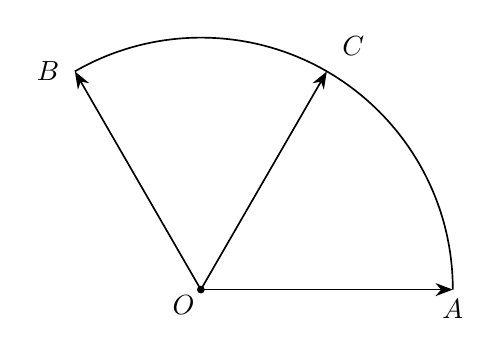
\begin{tikzpicture}[x=1cm,y=1cm,line width=.6pt,font=\normalsize]
\coordinate (O) at (0,0);
\coordinate (A) at (3.2,0);
\coordinate (B) at (-1.6,2.7713);
\coordinate (C) at (1.6,2.7713);
\draw (A) arc[start angle=0,end angle=120,radius=3.2cm];
\draw[-{Stealth[length=2.2mm]}] (O)--(A);
\draw[-{Stealth[length=2.2mm]}] (O)--(B);
\draw[-{Stealth[length=2.2mm]}] (O)--(C);
\node[below left=2pt,inner sep=0pt] at (O) {$O$};
\node[below] at (A) {$A$};
\node[left,xshift=-2pt] at (B) {$B$};
\node[above right,xshift=2pt,yshift=2pt] at (C) {$C$};
\fill (O) circle[radius=1.4pt];
\end{tikzpicture}
